\documentclass[12pt,a4paper,oneside]{report}
%\documentclass[12pt,a4paper,twoside,openright]{report}  % Duplex

\usepackage{xltxtra}
\usepackage{mathtools}
\usepackage{enumerate}
\usepackage{graphicx}
\usepackage{xcolor}
\usepackage[top=25mm,right=25mm,bottom=25mm,left=35mm]{geometry}
%\usepackage{fancyhdr}
\usepackage{lastpage}

\usepackage[hungarian,english]{babel}

\usepackage{sectsty}
\usepackage{setspace}
\usepackage[hang]{caption}
\usepackage{hyperref}
\usepackage{minted}

%------------------------------------------------------------------------------
% Main variables
%------------------------------------------------------------------------------
\newcommand{\vikszerzo}{Dányi Bence}
\newcommand{\vikkonzulens}{Gincsai Gábor}
\newcommand{\vikcim}{Social média analitika elosztott környezetben}
\newcommand{\viktanszek}{Automatizálási és Alkalmazott Informatika Tanszék}
\newcommand{\vikdoktipus}{Szakdolgozat}

%------------------------------------------------------------------------------
% Page layout setup
%------------------------------------------------------------------------------
% we need to redefine the pagestyle plain another possibility is to use
% the body of this command without \fancypagestyle and use \pagestyle{fancy}
% but in that case the special pages (like the ToC, the References,
% and the Chapter pages) remain in plane style.

\pagestyle{plain}
\setlength{\parindent}{0pt}
\setlength{\parskip}{8pt plus 3pt minus 3pt}

% \setcounter{secnumdepth}{0}
% \sectionfont{\large\upshape\bfseries}
\setcounter{secnumdepth}{2}
\onehalfspacing

%------------------------------------------------------------------------------
% Setup hyperref package
%------------------------------------------------------------------------------
\hypersetup{
    bookmarks=true,            % show bookmarks bar?
    unicode=false,             % non-Latin characters in Acrobat’s bookmarks
    pdftitle={\vikcim},        % title
    pdfauthor={\vikszerzo},    % author
    pdfsubject={\vikdoktipus}, % subject of the document
    pdfcreator={\vikszerzo},   % creator of the document
    pdfproducer={XeLaTeX},     % producer of the document
    pdfkeywords={keywords},    % list of keywords
    pdfnewwindow=true,         % links in new window
    colorlinks=true,           % false: boxed links; true: colored links
    linkcolor=black,           % color of internal links
    citecolor=black,           % color of links to bibliography
    filecolor=black,           % color of file links
    urlcolor=black             % color of external links
}

%------------------------------------------------------------------------------
% Some new commands and declarations
%------------------------------------------------------------------------------

% define references
\newcommand{\figref}[1]{\ref{fig:#1}.}
\renewcommand{\eqref}[1]{(\ref{eq:#1})}
\newcommand{\listref}[1]{\ref{listing:#1}.}
\newcommand{\secref}[1]{\ref{sec:#1}}
\newcommand{\tabref}[1]{\ref{tab:#1}.}

\newminted[js]{javascript}{fontsize=\footnotesize}
\newminted[jade]{jade}{fontsize=\footnotesize}
\newminted[html]{html}{fontsize=\footnotesize}
\newminted[sh]{sh}{fontsize=\footnotesize}
\newminted[css]{css}{fontsize=\footnotesize}
\newminted[stylus]{jade}{fontsize=\footnotesize}

\author{\vikszerzo}
\title{\viktitle}

\includeonly{
  % project,%
  titlepage,%
  declaration,%
  abstract,%
  introduction,%
  chapter1,%
  chapter2,%
  chapter3,%
}

%------------------------------------------------------------------------------
% Setup captions
%------------------------------------------------------------------------------
\captionsetup[figure]{
%labelsep=none,
%font={footnotesize,it},
%justification=justified,
width=.75\textwidth,
aboveskip=10pt}

\renewcommand{\captionlabelfont}{\small\bf}
\renewcommand{\captionfont}{\footnotesize\it}

%------------------------------------------------------------------------------
% Table of contents and the main text
%------------------------------------------------------------------------------
\begin{document}
\addtocontents{toc}{\protect\setstretch{0.9}}
\selectlanguage{hungarian}
\pagenumbering{arabic}
% %------------------------------------------------------------------------------
% Feladatkiiras (a tanszeken atveheto, kinyomtatott valtozat)
%------------------------------------------------------------------------------
\clearpage
\begin{center}
\large
\textbf{FELADATKIÍRÁS}\\
\end{center}

A közösségi média platformok rohamos terjedésével felmerült a kérdés
a felhasználók részéről, hogy a megosztott tartalmakat hogyan tudnák a lehető
leghatékonyabban eljuttatni a célközönségüknek.
A Twitter az egyik legnépszerűbb ilyen platform, a felhasználói pedig leginkább
olyan emberek, akik az őket érdeklő információkról valós időben, azonnal
szeretnének tudni.

A hallgató feladata egy olyan webes alkalmazás megírása Node.js környezetben,
ami a tartalmat megosztani kívánó felhasználó számára információt ad arról,
hogy mely időpontokban kell megszólítania a követőit, hogy a közölt tartalom
a lehető legtöbb felhasználóhoz eljusson.

A hallgató feladatának a következőkre kell kiterjednie:

\begin{itemize}
\item Mutassa be a felhasznált technológiákat.
\item Készítse el az alkalmazást JavaScript nyelven.
\item Tegye képessé a programot arra, hogy elosztott környezetben,
  hálózaton keresztül kooperálva egyszerre több példány is fusson belőle.
\item Az elkészült alkalmazás belső működését monitorozza, tegye mérhetővé.
\end{itemize}

\include{titlepage}
\tableofcontents\vfill
\include{declaration}
%------------------------------------------------------------------------------
% Abstract in hungarian
%------------------------------------------------------------------------------
\chapter*{Kivonat}\addcontentsline{toc}{chapter}{Kivonat}

A Twitter napjaink egyik legnépszerűbb kozösségi platformja, segítségével
egyszerűen tudunk taralmat megosztani másokkal. Azonban az üzenet gyakran
nem jut el a célközönségéhez, ha azt nem a megfelelő időben publikáljuk.

Erre a problémára nyújt megoldást az általam írt szoftver. Követőink
viselkedése alapján megbecsüli, hogy milyen időintervallumban célszerű
\emph{tweetelni}, ha potenciálisan a letöbb követőnkhöz szeretnénk eljuttatni
az üzenetünket.

Platformként a Node.JS-t választottam, mert pontosan az ilyen jellegű
feladatokban szerepel jól, hatékonyan képes skálázódni, beépített megoldások
segítik a hatékony elosztott működést.

A JavaScript napjaink egyik legnépszerűbb programozási nyelvve, számos
programozási paradigmát (objektum-orientált, funkcionális, stb.) támogat,
teljesítményben pedig már felveszi a versenyt az eddig egyeduralkodónak
gondolt natív társaival.

A legfőbb szempont a tervezés során az volt, hogy lazán csatolt, könnyű
komponensekből építsem meg a rendszert, hiszen a jól skálázható, eloszott
működéshez ez elengedhetetlen.

\vfill

\selectlanguage{english}

%------------------------------------------------------------------------------
% Abstract in english
%------------------------------------------------------------------------------
\chapter*{Abstract}\addcontentsline{toc}{chapter}{Abstract}

Twitter is one of the most popular social networks, people can
easily share content with others. This method of content sharing can be very
efficient, albeit it heavily depends on the time of the publishing.

My software addresses this problem by analysing the behavior of our follower
base. After this step, the application tells us when should we publish our
content to maximize the number of impressions.

My chosen platform was Node.JS, because it is designed for these kind of
applications. It scales well, one can write distributed network applications
very easily.

The JavaScript language is very popular, it supports various programming
paradigms (object-oriented, functional, etc.), its performance is very
impressive, it is comparable to native languages like C++, Java, C\#.

My top priority during the development was that the individual software
components should be loosely coupled and lightweight. These properties
are necessary for a scalable, distributed system.

\vfill

\selectlanguage{hungarian}

%------------------------------------------------------------------------------
\chapter{Bevezető}
%------------------------------------------------------------------------------

\section{A megoldandó probléma}

A Twitter közösségi platform segítéségével a felhasználók rövid szöveges
(maximum 140 karakteres) tartalmakat tudnak megosztani egymással.
Az átlagos felhasználó valamilyen mobil eszközön használja a szolgáltatást.
\cite{About-Twitter}

Mivel a közölt tartalmak (\emph{tweetek}) nagyon rövidek, a felhasználók
sokkal többet is tweetelnek, mint mondjuk egy blog esetén.
A tipikus felhasználó csak az elmúlt néhány óra eseményeit tudja követni
(vagy még kevesebbet), hiszen egész egyszerűen az információ sokkal
gyorsabban áramlik, mint ahogy a felhasználó azt fel tudná dolgozni.

Pontosan emiatt nagyon nehéz a platformot információk hatékony, gyors
terjesztésére használni. Egy tweet nagyon gyorsan elveszik az információk
rengetegében, több tweet azonban negatívan hat azokra a felhasználókra,
akik folyamatosan követik az eseményeket.

Az általam írt szoftver ezt a problémát próbálja meg megoldani úgy,
hogy a felhasználó követő bázisának szokásait elemezve megmondja azt az
idő intervallumot, amikor a tweet a legtöbb emberhez eljuthat.
Mivel a tweetek nézettségét mérni nagyon limitáltan lehet,
a rendszer gyakorlatilag fekete dobozként viselkedik,
így azt az egyszerű hipotézist állítottam föl,
hogy a legideálisabb időpont az, amikor a legtöbb felhasználó online,
azaz épp a Twittert használja valamilyen felületen keresztül.
Ez szintén nem mérhető közvetlenül, így online felhasználónak az számít,
aki éppen tweetelt (pl. az elmúlt 15 percben).

Természetesen ez a heurisztika nem pontos, hiszen nem foglalkozik azokkal,
akik nem tweetelnek, vagy esetleg szeretik akár több napra visszamenőleg
átolvasni az falukat. Ezek olyan tényezők, amiket közvetlenül nem,
közvetve is csak nagyon körülményesen lehet mérni, ezeknek a szokásoknak
a figyelembevétele messze túlmutat a dolgozat keretein.

\section{Szükséges lépések a megoldáshoz}

A probléma ismeretében a következő részproblémákat határoztam meg,
amiket a programnak meg kell oldania:

\begin{itemize}
  \item A szoftvernek rendelkeznie kell egy webes felülettel, amin keresztül a
felhasználó azonosítása megtörténhet.
  \item A szükséges adatokat \emph{on-demand} jelleggel nem lehet lekérdezni,
mert hosszadalmas folyamat, így szükség van a háttérben futó feldolgozó
egységekre.
  \item Az elosztott működést koordinálni kell, az egyes komponenseknek
kommunikálniuk kell egymással, ezt az összekötő réteget is meg kell valósítani.
  \item A folyamatok monitorozása fontos a rendszer elemzéséhez, így
szükséges egy rugalmas naplózó rendszer integrálása.
\end{itemize}

\section{A dolgozat felépítése}

A dolgozat második fejezetében ismertetem a rendelkezésre álló technológiákat,
azok szerepét a megvalósításban, röviden ismertetem a főbb tulajdonságaikat,
illetve megindoklom, hogy miért döntöttem az adott technológiák mellett,
esetenként összehasonlítva más alternatívákkal őket.

A harmadik fejezetben ismertetem az alkalmazás egyes tervezési döntéseit,
a lehetséges alternatívákkal együtt. Kitérek a felmerülő technikai problémákra,
illetve bemutatom a konkrét szoftvert feladatban kitűzött
problémák megoldására.

Az utolsó fejezet néhány mérési eredményt mutat be a rendszer működéséről,
illetve kitekintés, hogy hogyan lehetne további funkciókkal kiegészíteni
a rendszert, milyen további előnyök származnának belőle.

\chapter{Felhasznált technológiák}

\section{JavaScript}

A JavaScript egy dinamikus, gyengén típusos nyelv, amit Brendan Eich
fejlesztett ki 1995-ben \emph{Mocha} kódnéven, megjelenésekor LiveScript néven,
és a Netscape böngészőben nyújtott támogatást különböző felhasználói
interakciókhoz.\cite{JSAnnounce}

Szintaktikáját tekintve a C-típusú nyelvek közé sorolható (ahogy a C++, Java és
C\# is), azonban ezektől eltérően az öröklési modellje nem osztály, hanem
prototípus alapú. Ez a különbség sok félreértésre ad okot a nyelv használóinak
körében, megítélése pont emiatt nagyon szélsőséges.

A nyelvet később az Ecma International karolta fel, ami azóta is karbantartja
a nyelv specifikációját.

\subsection{ECMAScript}

Az ECMAScript a JavaScript nyelv specifikációja (a JavaScript név hivatalosan
a Mozilla tulajdona, így valójában a ma elterjedt nyelvre ECMAScript néven
lenne helyes hivatkozni), aminek a sorsáról a TC39 (Technical Committee)
csoport tagjai döntenek.\cite{TC39}

A tagok különböző, főleg IT-val foglalkozó vállalatok által delegált mérnökök,
többek között Google, Intel, Microsoft, Mozilla, Apple, eBay
alkalmazottak.
A nyelv ettől függetlenül a felhasználók aktív közreműködésével készül,
bárki tehet javaslatokat a specifikációt illetően (pl. a specifikáció hivatalos
levelezőlistáján\cite{ESDiscuss}).

\subsubsection{ECMAScript 1}

Az első verzió\cite{ECMAScript-1} 1997-ben jelent meg, gyakorlatilag csak egy
formális specifikációt nyújtott a már meglévő nyelv számára,
így más böngészőkben is azonos működésű nyelvet lehetett implementálni.

\subsubsection{ECMAScript 3}

A második verzió túl sok újdonságot nem tartalmazott, az ECMAScript 3 azonban
számos új nyelvi elemet vezetett be\cite{ECMAScript-3}, többek között
a \verb=try{ } catch(e) { }= szerkezetet, illetve a reguláris kifejezéseket.

A ma használt összes böngésző teljes támogatást nyújt a nyelvhez.

\subsubsection{ECMAScript 4}

A következő verzió olyan sok új elemet tartalmazott, hogy végül sokat közülük
véglegesen elvetettek, másokat a \emph{Harmony} projectbe helyeztek át,
amiből később a 6-os és 7-es verziók merítettek ötleteket.
A specifikáció soha nem készült el teljesen.

\subsubsection{ECMAScript 5}

A 2009-ben elkészült specifikációt a ma használt szinte összes modern böngésző 
támogatja (vagy a javított, 5.1-es változatot\cite{ECMAScript-5}).
A 3-as verzióhoz képest tartalmazza a getterek, setterek specifikációját,
natív JSON támogatást, illetve egységesítette a korábban használt
reflection módszereket.

Tartalmazza az ún. \emph{strict} módot, amivel a leggyakrabban elkövetett
hibákat statikus analízis eszközökkel ki lehet szűrni már a fejlesztés korai
szakaszában.

\subsubsection{ECMAScript 6}

Jelenleg is fejlesztés alatt áll\cite{ECMAScript-6},
jelentős újdonságokat tartalmaz, az egyik legnagyobb újítás az osztályok
és modulok bevezetése, generátorok, beépített \verb=Map=, \verb=Set=,
\verb=WeakMap= adatszerkezetek, a metaprogramozáshoz nélkülözhetetlen
\verb=Proxy=-k.

Jelenleg a böngészők csak részben támogatják, ám folyamatosan zajlik az átállás.
Az általam megírt szoftver erőteljesen épít a generátorokra.

Különböző eszközökkel az ES6 kód ES5-re fordítható (pl. Traceur, 6to5), így
az új verzióban írt kódot is lehet futtatni a mai böngészőkben.
Pl. az AngularJS 2.0 az elsők között lévő keretrendszer,
ami már teljesen ezekre az új alapokra épít.

\subsubsection{ECMAScript 7}

A fejlesztés korai stádiumában van, a tervek között szerepel az \emph{operator
overloading} támogatása, érték típusok (saját primitív típusok), \verb=async=
függvények, mintaillesztés.

\section{Node.js}

A Node.js a Google által fejlesztett \emph{v8} JavaScript értelmezőt használó
JavaScript futtatókörnyezet\cite{Node}, ami a Ruby-ból ismert Event Machine
\cite{EventMachine} és a Python Twisted\cite{Twisted} moduljához hasonlóan
működik, ám a felhasználó elől teljesen elrejti az \emph{eseményhurkot}
(\secref{async-io}. fejezet).

Az első verziót Ryan Dahl írta 2009-ben, azóta a projekt vezetése TJ Fontaine
kezébe került\cite{Node-TJ}, jelenleg is fejlesztés alatt áll, a következő stabil verziója
a v0.12 lesz. A szakdolgozatban elkészített szoftver a node 0.11-es verzióján
fut, mivel sok olyan funkciót használ, ami a stabil ágon (0.10) nem elérhető.

A Node.js-t már számos nagyvállalat használja, ami képes a régi,
rugalmatlan Java (vagy .NET) alapú stack kiváltására.
Az egyik legnagyobb sikertörténet a PayPalhoz fűződik, ahol a frontend
szoftvert (a PayPal webes felületét) újraírták Java és Node.js alapokon is.
\cite{PayPal-Case}

A kísérlet során két ugyanolyan funkcionalitással (azonos specifikációval)
rendelkező szoftver implementáltak Java-ban és Node-ban. Az eredény:
az utóbbit fele annyi mérnök fele annyi idő alatt fejezte be,
a kész szoftver pedig kétszer annyi HTTP kérést bírt kiszolgálni
másodpercenként, mint az ekvivalens Java alkalmazás
(a válaszidő is javult a harmadával), a Node.js verzió pedig nem is
használta ki a Java verzióval ellentétben a többmagos környezet előnyeit.

\subsection{Aszinkron IO}\label{sec:async-io}

A Node.js a grafikus rendszerekben megszokott \emph{eseményhurok}-ra épít,
azaz egy végtelen ciklusban várakozik eseményekre, majd azokat a megfelelő
\emph{callback} függvényeknek továbbítja.

A platformon alapvetően minden IO-t érintő hívás aszinkron,
azaz a függvényhívás nem blokkol, hanem az IO művelet befejezése után
a megadott \emph{callback} függvény fut le. Természetesen lehetőség van
szinkron végrehajtásra is, azonban ezeket egyszerű konzolos
alkalmazásokhoz érdemes csak használni.

Szemléltetésképpen egy szinkron hívás:

\begin{js}
var result = http.get('http://nodejs.org');
\end{js}

A \verb=http.get= függvény itt blokkol, azaz addig, amíg a művelet nem
fejeződik be, a program nem tud tovább futni, ``lefagy''.
Ezt elkerülendő, a Node az aszinkron működést támogatja:

\begin{js}
http.get('http://nodejs.org', function(err, result) {
  // hiba, illetve az eredmény kezelése
});
\end{js}

A \verb=http.get= itt rögtön visszatér (végül pedig az eseményhurokban fog
várakozni az alkalmazás), és ha megérkezett a válasz(esemény),
a futtatókörnyezet lefuttatja a hozzárendelt \emph{callback} függvényt.

Hagyományos szinkron hívásoknál ha több \verb=get= hívást szeretnénk
végrehajtani, akkor az egyetlen lehetőségünk a szálak használata.
A szálak nem skálázhatóak, erőforrás-pazarlóak (rengeteg memóriát igényelnek,
mivel saját \emph{stack}-re van szükségük).
Egy node folyamat képes akár párhuzamosan több tízezer HTTP kérést
is kiszolgálni, a hagyományos, thread pool alapú megoldással ez
elképzelhetetlen.
Volt már rá példa, hogy egyetlen node folyamat egymillió TCP kapcsolatot
tartott fönn\cite{Node-1M}, mindössze 16GB memóriát igényelve.
Szál-alapú megoldással ugyanehhez 4TB memóriára volna szükség (amennyiben
az átlagosnak mondható 4MB-os stack mérettel számolunk)

A megoldás hátránya a bonyolultabb kód, erre a problémára a generátorok
jelentik a megoldást (\secref{async}. fejezet).

Az egyszálú működés másik hátránya, hogy a különösen CPU-intenzív feladatokra
nem célszerű használni, hiszen bár az IO hívások aszinkronak, a többi
művelet szinkron, így egy sokáig blokkoló (CPU-t használó) kérés miatt az
utána érkező kérések addig nem kerülnek kiszolgálásra, amíg az előző be nem
fejeződött, nem tapasztaljuk a szálaknál megszokott preemptív működést.

A problémára részben megoldást nyújthat, ha több node kiszolgáló folyamatot
indítunk el (pl amennyi processzor rendelkezésre áll a rendszeren), ezzel
az egyszálú működés hatékonyságán javítottunk, azonban a node nem-preemptív
természetén nem változtat.

Természetesen létezik megoldás arra, hogy szálakat használjunk: natív modulokat
kell írnunk (C++-ban), vagy egy erre specializált modult használnunk,
amivel JavaScriptet futtató szálakat tudunk létrehozni, ez utóbbira példa
a \verb=threads_a_gogo= könyvtár.\cite{Threads-a-gogo}
Jelen szakdolgozatnak nem célja ezeket a
megoldásokat bemutatni, így a továbbiakban mindig egyszálú működést lehet
feltételezni.

\subsection{CommonJS modulok}

A node programok modulokból épülnek fel, amik a CommonJS specifikációt követik
\cite{CommonJS}.
Minden modul a következő struktúrát mutatja:

\begin{js}
var beep = require('beep');

module.exports = function beepboop() {
  beep();
  console.log('boop');
};
\end{js}

Azaz meglévő modulokat a \verb=require= függvénnyel tudunk beimportálni,
a modul által nyújtott API-t pedig a \verb=module.exports=
(illetve \verb=exports=) változón keresztül tudjuk módosítani.

\subsection{npm}

A node szerves része a beépített csomagkezelő, az \verb=npm=, amivel a
felhasználók által írt modulokat tudjuk telepíteni, illetve magunk is
publikálhatunk modulokat. Jelen sorok írásakor az \verb=npm= csomagok száma
már átlépte a 100000-t\cite{NPM-100K},
ez több, mint bármelyik másik csomagkezelő rendszerben lévő csomagok száma
(a második legnagyobb a Java Maven, körülbelül 80000 csomaggal).

Egy csomag az

\begin{sh}
$ npm install [név]
\end{sh}

paranccsal telepíthető.

A csomagok része a \verb=package.json= fájl, ami metainformációkat tartalmaz a
csomagról: név, verzió, függőségek, a részletes leírás megtalálható az
\verb=npm= oldalán\cite{Package-JSON}.

\subsection{Szemantikus verziókezelés}

Az \verb=npm= modulok az ún. \emph{semantic versioning}-et követik\cite{Semver},
ez azt jelenti, hogy a modul három verziószámmal rendelkezik:

\begin{description}
\item[major] Fő verzió szám, az azonos számmal rendelkező release-ek garantáltan
azonos API-val rendelkeznek, így a csomagok frissítése egyszerűen
automatizálható
\item[minor] Alverzió, a visszafelé kompatibilis változásokat lehet ennek a
számnak a növelésével jelezni.
\item[patch] A kisebb hibajavítások után célszerű ezt a számot növelni.
\end{description}

Amennyiben a publikált modulok betartják ezeket a konvenciókat, úgy
a csomagfrissítések automatizálhatóak, hiszen a modul bármikor magasabb
\emph{minor} verzióra frissíthető, mert az garantáltan visszafelé kompatibilis.

\section{\texttt{browserify}}

A nagyobb méretű webes kliensoldali alkalmazások egyik nagy problémája,
hogy a JavaScript nyelvi szinten nem ismeri a \emph{modul} fogalmát
(bár jelenleg az ES6 részeként már kidolgozás alatt áll a
specifikáció\cite{ES6-Modules}),
így komplex szoftverek csak rendkívül kényelmetlenül írhatók benne.

A problémára több megoldás is született, mindkét megközelítés a modul fogalmát
ragadja meg, ezek közül az egyik a CommonJS, a másik pedig az AMD
(Asynchronous Module Definition) specifikáció.
Mindkettőre létezik több implementáció is (AMD API-t biztosít pl. a RequireJS).

Mivel Node.JS környezetben a CommonJS a megszokott modul-implementáció, így
kézenfekvő, hogy az alkalmazás kliens-oldali részéhez is érdemes ezt használni,
ennek számos előnye van : pl. kódmegosztás, illetve maga a tény, hogy szinte
ugyanaz a rendszer van mind kliens mind szerver oldalon (így az npm-ben lévő
több tízezer csomag képes a böngészőben is futni).

Az egyik legnépszerűbb eszköz a CommonJS modulok \emph{becsomagolására}
a \verb=browserify=\cite{Browserify},
ami képes a program minden függőségét egyetlen JavaScript fájlba csomagolni:

\begin{sh}
$ browserify app.js -o bundle.js
\end{sh}

Ahol az \verb=app.js= az alkalmazás belépési pontja, a \verb=bundle.js=
pedig a kimeneti fájl. A program felderíti az alkalmazás függőségeit,
azokat a megfelelő wrapper függvényekbe csomagolja, majd konkatenálja.

\subsection{Inkrementális fordítás}

Mivel a fordítási folyamat adott esetben néhány másodpercig is tarthat,
így érdemes a \verb=watchify= csomagot\cite{Watchify}
használni, ami képes az inkrementális fordításra,
illetve a fájlok változása esetén automatikusan újrafordítja
az alkalmazást, gyakorlatilag néhány milliszekundum alatt:

\begin{sh}
$ watchify app.js -o bundle.js
\end{sh}

A fordítási folyamat egyszerűen bővíthető pluginekkel, így a lefordított
fájlhoz akár \emph{source map} is rendelhető, amivel a fordítás miatt
keletkező debugolási problémák (nem lehet visszakövetni, hogy a lefordított,
és akár minifikált fájlban az egyes szimbólumok hol vannak a forrásfájlokban)
gyakorlatilag megszűnnek.

\subsection{Sablonkezelés}

Az alkalmazásoknál gyakori, hogy az egyes DOM elemek dinamikusan generálódnak,
ekkor szükség van valamilyen \emph{template} fájlra, amibe különféle változókat
behelyettesítve megkapjuk a végleges HTML kódot.

Erre a célra a Jade könyvtárat\cite{Jade} használtam,
ami HTML kód generálására képes, és nagyon elegáns szintaxissal rendelkezik:

\begin{jade}
doctype html
html
  head
    title Teszt
  body
    h1 Hello world
    a(href='http://nodejs.org') Ez egy link
\end{jade}

Aminek az eredménye fordítás után:

\begin{html}
<!DOCTYPE html>
<html>
  <head>
    <title>Teszt</title>
  </head>
  <body>
    <h1>Hello world</h1><a href="http://nodejs.org">Ez egy link</a>
  </body>
</html>
\end{html}

Természetesen vezérlési szerkezetek is használhatók:

\begin{jade}
h1 Teendők:
ul
  each item in list
    li
      span!= item.name
      if item.done
        span (kész)
\end{jade}

Az elkészült \verb=.jade= kiterjesztésű fájlok kliens oldalon egyszerűen
felhasználhatóak a \verb=jadeify= segítségével: a kívánt sablon egy egyszerű
\verb=require= hívással betölthető, \verb=browserify= által lefordított
fájlba automatikusan bekerül a sablon optimalizált, végrehajtható változata:

\begin{js}
var template = require('template/todo.jade');
var todoList = [{
  name: 'Foo',
}, {
  name: 'Bar',
  done: true,
}];

document.body.innerHTML = template(todoList);
\end{js}

A jade sablonnyelv adatkötési réteget nem biztosít, ha erre is szükség van,
akkor érdemes külső megoldást használni, ilyen a Facebook által fejlesztett
React (létezik jade integráció is, a \verb=react-jade= csomagot
kell telepíteni).

A kliens oldali logika nem indokolta a bonyolult adatkötéseket, így az
elkészült szoftverben csak statikus jade sablonokat használtam.

\section{A \texttt{co} könyvtár}

Az aszinkron működés egyik legnagyobb hátránya, hogy az elkészült program
nehezen átlátható, gyakori az ún. \emph{callback hell} jelenség:

\begin{js}
asyncOp(function() {
  asyncOp(function() {
    asyncOp(function() {
      done();
    });
  });
});
\end{js}

A probléma megkerülésére több megoldás is létezik, a gyakorlatban a
\emph{Promise} illetve a \emph{generátor} alapú megközelítést alkalmazzák.

Az előbbi nem igényel új nyelvi elemet, azonban rendkívül sok \emph{boilerplate}
kóddal jár:

\begin{js}
asyncOp().then(function() {
  return asyncOp();
}).then(function() {
  return asyncOp();
}).then(done);
\end{js}

Pont az ilyen problémák miatt döntöttem amellett, hogy a generátor-alapú
megközelítést használjam az elkészített alkalmazásban.
Ennek használatát könnyíti meg a \verb=co= könyvtár.

\subsection{Generátor függvények}

Az ECMAScript 6 egyik legnagyobb újdonsága a generátorok bevezetése,
amelyek a C\# \verb=yield=\cite{CSYield} kulcsszavához hasonló működést
produkálnak.
Segítségével képesek vagyunk a lusta kiértékelést használva
potenciálisan végtelen szekvenciákon végigiterálni.

\begin{js}
function* squares() {
  for(var i = 1;; i++) {
    yield i * i;
  }
}

for(var n of squares()) {
  if (n > 100) {
    break;
  }
  console.log(n);
}
\end{js}

A példakódban a \verb=function*= kulcsszó jelzi, hogy egy generátor függvényt
definiálunk, a függvény pedig az összes négyzetszámot generálja
(ami természetesen egy végtelen szekvencia). A \verb=for-of= konstrukcióval
a generátor értékein tudunk végigiterálni.
Mivel egy végtelen hosszú listát nem tudunk kiértékelni, az első 10
négyzetszám után megszakítjuk a futást.

Az iterációt megkönnyítő \verb=for-of= csak szintaktikus édesítőszer,
a generátort magunk is léptethetjük a \verb=next()= metódussal:

\begin{js}
var s = squares();
for(;;) {
  var result = s.next();
  if (result.done || result.value > 100) {
    break;
  }
  console.log(result.value);
}
\end{js}

Elsp lépésként példányosítjuk a generátort (szintaktikailag ez megegyezik
a függvényhívással), majd a generátorpéldányt léptetjük a \verb=next()=
metódussal. Ekkor megkapjuk a generátorban a \verb=yield= által kiszámolt
értéket (\verb=result.value=). Ha a generátort nem lehet tovább léptetni,
a \verb=result.done= változóba \verb=true= érték kerül.

\subsection{Aszinkron működés generátorokkal}\label{sec:async}

Sajnos a nyelv a C\#-ban ismert \verb=async-await= konstrukciót nem támogatja
(feltehetően csak az ES7-ben lesz a nyelv része),
azonban a megfelelő \emph{wrapper} függvény meghívásával ahhoz nagyon hasonló
működés emulálható, azaz a megfelelő helyen (aszinkron függvényhívásoknál)
a futás felfüggesztődik, az eseményhurok képes más feladatokat végrehajtani,
majd ha a művelet befejeződött, a vezérlést visszakerül a megfelelő helyre.

Ehhez a már meglévő aszinkron függvényeinket kell becsomagolni úgy,
hogy azok ne vegyenek át \emph{callback} függvényt, hanem egy ún.
\emph{thunk}-ot adjanak vissza, amit aztán a megfelelő modul képes meghívni.

\begin{js}
function thunkify(fn) {
  var args = [].slice.call(arguments);
  var thisArg = this;
  return function thunk(cb) {
    return fn.apply(thisArg, args.concat[cb]);
  };
}
\end{js}

A \verb=thunkify= függvény egy becsomagolandó függvényt (\verb=fn=) vár,
és a becsomagolt függvényt (\verb=thunk=) adja vissza. Ezzel tulajdonképpen
\emph{lekötjük} a függvény első $n$ argumentumát.

A \verb=thunk=-ot generálva a generátort futtató modul egy speciális
callback függvénnyel hívja meg, ami pusztán arra szolgál,
hogy a generátort tovább léptesse.
Ennek a lehető legegyszerűbb megvalósítása:

\begin{js}
function run(gen) {
  var instance = gen();
  function cont(thunk) {
    thunk(function (err, result) {
      var ret;
      if (err) {
        ret = instance.throw(err);
      } else {
        ret = instance.next(result);
      }
      if (ret.value) {
        cont(ret.value);
      }
    });
  }
  cont(instance.next().value);
}
\end{js}

Az általam írt \verb=genzen= könyvtár hasonló funkcionalitást nyújt,
ám nem csak \emph{thunk}-ot fogad el, hanem \emph{promise}-t is,
a szakdolgozatban azonban a \verb=co= modult\cite{Co} használom,
mivel támogatja a párhuzamosítást, illetve mert rengeteg modul érhető el hozzá.

Használata nagyon egyszerű:

\begin{js}
function sleep(ms) {
  return function (cb) {
    setTimeout(cb, ms);
  }
}

co(function* () {
  console.log(1);
  yield sleep(1000);
  console.log(2);
});
\end{js}

A példában a két \verb=console.log= hívás 1000ms különbséggel hívódik meg.

A modul támogatja a párhuzamosságot:

\begin{js}
  co(function* () {
    var pages = yield [
      http.get('https://nodejs.org'),
      http.get('https://npmjs.org'),
    ];
    console.log(pages);
  });
\end{js}

A példában a \verb=pages= változó értékébe a felsorolt két honlap tartalma
kerül, a letöltés párhuzamosan történik, a művelet végén a szinkronizációt
is megoldja a modul.

\section{\texttt{koa}}

A node legelterjedtebb webes keretrendszere az \verb=express=\cite{Express}
framework, ami a beépített \verb=http= modulra (webszerver) épül,
és kibővíti azt kényelmes routing lehetőségekkel,
illetve ún. \emph{middleware}-ek használatával szabhatjuk testre a működését.

A \verb=koa=\cite{Koa} ennek a következő generációs megfelelője,
elődjéhez képest sokkal letisztultabb, elegánsabb interfészt nyújt,
szinte teljesen a fejlesztőre bíz minden fontos architekturális döntést,
az aszinkron működéshez a \verb=co= modult és generátorokat használ.

\subsection{Middleware-alapú architektúra}

A \verb=koa= esetében a middleware egy egyszerű generátor, aminek a feladata
az érkező kérés lekezelése, majd a vezérlés továbbadása a következő
middleware rétegnek, majd végül az érkező válasz további manipulálása.
Természetesen egyik lépés sem kötelező, minden logika implementálása a
fejlesztőre van bízva. Egy tipikus middleware (ez esetben egy naplózó)
felépítése:

\begin{js}
var koa = require('koa');
var app = koa();

app
  .use(function* log(next) {
    var start = Date.now();
    yield* next;
    console.log(
      'Request to %s took %d ms',
      this.url,
      Date.now() - start
    );
  });
\end{js}

Első lépés az alkalmazás létrehozása, majd az alkalmazáshoz hozzáadjuk az
általunk megírt middleware-t a \verb=use= metódussal.
A generátor egyetlen paramétert vár (\verb=next=), amivel a vezérlést
tovább tudjuk adni a soron következő rétegnek.
A példa middleware egyszerű naplózást valósít meg, a szabványos kimenetre
írja az érkező HTTP kéréseket, illetve a hozzájuk tartozó válaszidőt.
Elsőként eltároljuk az aktuális időbélyeget (``leszálló'' ág),
majd a \verb=yield* next= utasítással delegáljuk a következő generátornak a
vezérlést (a \verb=yield*= kulcsszó nem szakítja meg a generátor futását,
csak tovább delegálja azt), végül a ``felszálló'' ágon elvégzi a szükséges
naplózást (\verb=console.log= hívás).
A működésre az egyik legszemléletesebb analógia a böngészők DOM eseménykezelése,
ahol a \verb=yield* next= előtti rész az esemény \emph{capture} fázisának,
az azutáni rész pedig a \emph{bubble} fázisnak felel meg.

Természetesen léteznek ennél egyszerűbb middleware-ek, egy \emph{hello world}
alkalmazás szerkezete az alábbi:

\begin{js}
var koa = require('koa');
var app = koa();

app.use(function* hello() {
  this.body = 'Hello world!';
});
\end{js}

A \verb=this= jelenti a HTTP kérés kontextusát, a \verb=body= adattag pedig
a kérésre adott választ jelenti. Ez lehet egy egyszerű \verb=String=, de akár
JSON objektum is, ekkor a megfelelő HTTP válasz fejléc is beállítódik
(\verb=Content-Type: application/json=), az objektum pedig szerializálódik.
A válasz opcionálisan akár \verb=Stream= is lehet, ez akkor lehet hasznos,
ha pl. fájlokat szeretnénk kiszolgálni, és a teljes eredményt nem kívánjuk
(vagy nem is tudjuk) a memóriában tárolni, hanem folyamatosan szeretnénk
a kliensnek továbbítani.

\subsection{Általános struktúra}

A \verb=koa= alkalmazások maguk is middleware-ként viselkednek,
így azokat egyszerűen tudjuk egymásba ágyazni.
Az általános konvenció az, hogy egy fő alkalmazásba felvesszük a közösen
használt modulokat, majd azok alá felvesszük a megfelelő route-okon hallgató
önálló alkalmazásokat, így az elkészült szoftver laza csatolású, hiszen
a használt alkalmazások tetszőlegesen válogathatóak össze, azokat könnyen
fel lehet használni újra.

A \verb=koa= beépítetten csak egyetlen middleware-t (\verb=respond=) tartalmaz,
aminek a feladata pusztán a kéréshez tartozó kontextus inicializálása, illetve
egy 404-es hibakód visszaadása, ha egyik további middleware sem kezelte
le a kérést (nem állított be választ).

\subsection{Routing megoldások}

Természetesen a fejlesztő megírhatja a saját routing modulját,
azonban rendelkezésre állnak kész megoldások, amik ezt nagyban megkönnyítik.
Ezek közül az egyik a \verb=koa-route= modul, ami a megfelelő HTTP
metódusokra illeszkedő middleware generátorfüggvényeket gyárt az általunk
megadott kontrollerhez

\begin{js}
var koa = require('koa');
var route = require('koa-route');
var get = route.get;
var app = koa();

app
  .use(get('/users/:id', showUser));
\end{js}

A \verb=get= függvény paraméterként egy sztring mintát,
illetve egy middleware-t vár, és egy olyan middleware-t ad vissza,
ami a megfelelő mintára illeszkedő HTTP kéréseket továbbítja az átadott
kontrollernek (paraméterként pedig átadja az illesztett \verb=id= paramétert),
minden mást kérést átenged a soron következő middleware-nek.

A másik modul a \verb=koa-mount=, ezzel komplett \verb=koa= alkalmazásokat
tudunk URL-transzparens módon egymásba illeszteni, azaz az egyes
alrendszereknek nem kell tudnia teljes URL-ről.

\begin{js}
var mount = require('koa-mount');

users
  .use(get('/:id', showUser));

messages
  .use(get('/:id', showMessage));

app
  .use(mount('/users', users))
  .use(mount('/messages', messages));
\end{js}

A példában két \verb=koa= alrendszert (\verb=users= és \verb=messages=)
fogunk össze, melyek a \verb=/users= illetve a \verb=/messages= útvonalakon
hallgatnak. Az egyes alkalmazások nem tudnak (nem is tudhatnak) a
teljes elérési útról. A modult használva tetszőleges alkalmazások fűzhetőek
össze anélkül, hogy a moduljuk kódját módosítani kéne, így az eredmény
egy lazán csatolt, könnyen bővíthető architektúra.

\subsection{REST API}

A \emph{REST}\cite{REST} (Representational state transfer) egy konvenció a HTTP fölött
történő kommunikációra. A rendszerben erőforrásokat definiálunk
(pl. \emph{felhasználó}, \emph{üzenet}, stb.), ezekhez azonosítót rendelünk,
az erőforrásokat pedig ezen az URI-n (Uniform Resource Identifier) tudjuk
elérni, illetve manipulálni. Erre szolgálnak a különböző HTTP metódusok:

\begin{description}
  \item[GET] Adott erőforrás (vagy erőforrások) elérésére szolgál.
    Idempotens művelet, azaz a kimenete mindig ugyanaz, a meghívások számától
    függetlenül, és biztonságos is, az erőforrást nem módosítja, manipulálja.
  \item[POST] Új erőforrást hoz létre, nem idempotens.
  \item[DELETE] Adott erőforrást töröl, idempotens, de nem biztonságos, hiszen
    módosítja az erőforrást.
  \item[PUT] Az erőforrás \emph{teljes} leírását frissíti, idempotens, de nem
    biztonságos művelet.
  \item[PATCH] Az erőforrást \emph{részlegesen} frissíti, ugyanazon
    tulajdonságokkal rendelkezik, mint a PUT metódus.
\end{description}

Ezek a műveletek mind jól lefordíthatóak a rendszerben lévő modellek
metódushívásaira, így célszerűnek láttam, hogy ezeket a nagyon hasonló
műveleteket mind kiemeljem paraméterezhető middleware-kbe, amiket az alkalmazás
fejlesztése során többször is újra fel lehet használni.

Ilyen jellegű művelet a \emph{resolve}, ami a megadott (\verb=/resource/:id=)
alakú URI-ket képes feloldani valódi erőforrásokra:

\begin{js}
module.exports = function (name, resolver) {
  return function* resolve(id, next) {
    this[name] = yield* resolver(id);
    yield* next;
  };
};
\end{js}

\section{Stylus}

A böngészőben történő korszerű megjelenéshez szükség van CSS stílusfájlokra,
azonban a leírónyelv meglehetősen kényelmetlen, így helyette a CSS-re forduló
Stylus\cite{Stylus} nyelvet használtam.

A szintaxis támogatja az egymásba ágyazott CSS szelektorokat, illetve
számos programozási nyelvi eszköz érhető el benne
(változók, ciklusok, elágazások, függvények, stb.),
de a legnagyobb erénye, hogy rendkívül kompakt:

\begin{stylus}
body
  font-size 16pt
  h1
    color red
\end{stylus}

A fenti kódból a \verb=stylus= bináris az alábbi CSS kódot generálja:

\begin{css}
body {
  font-size: 16pt;
}
body h1 {
  color: #f00;
}
\end{css}

Maga a fordító szintén Node.JS alapú, az egyszerű fordításon kívül
természetesen a fejlesztést nagyban megkönnyítő automatikus fordítást is
támogatja:

\begin{sh}
  $ stylus --watch style.styl -o style.css
\end{sh}

\section{LevelDB}

A LevelDB a Google által fejlesztett beágyazható \emph{key-value} adatbázis
könyvtár\cite{LevelDB}.
Maga az adatbázis egy \emph{Map} adatszerkezet, ahol mind a kulcs,
mind az érték tetszőleges byte-sorozat.

3 alapvető műveletet támogat, \verb=put(key, value)=, \verb=get(key)= és
\verb=delete(key)=, ezen felül képes több műveletet egy atomi műveletként
végrehajtani, illetve a kulcsokon képes előre és hátrafelé iterálni.

A megszokott relációs adatmodellt nem támogatja, az indexelés is csak a kulcsra
megoldott, így minden bonyolultabb funkcionalitást a fejlesztőnek kell
megvalósítania.

Mivel az adatbázis nagyon egyszerű felépítésű, a teljesítménye a hagyományos
SQL adatbázisokhoz képest várhatóan nagyságrendekkel jobb.
Az általam írt szoftverben az adatok jellege nem követeli meg a relációs
adatmodellt, így inkább a teljesítményt választottam a kényelemmel szemben.

\section{InfluxDB}

Az InfluxDB egy ún \emph{time-series} adatbázis, ami elsősorban időfüggő
metrikák hatékony tárolására és elemzésére alkalmas\cite{InfluxDB}.
Az adatokat lehetőség van különböző adatbázisokban perzisztálni,
többek között akár LevelDB-n is.

A szoftver lehetőséget nyújt a tárolt adatok komplex elemzésére, egy SQL-hez
hasonló lekérdező nyelv segítségével, illetve a lekérdezés eredménye grafikusan
is megjeleníthető, így egyszerű diagramok készítése beépítetten támogatott.

Pl. ha szeretnénk perc felbontású adatokat kapni az alkalmazás átlagos
válaszidejéről az elmúlt egy órából, az alábbi lekéréssel tehetjük meg:

\begin{verbatim}
select mean(response_time)
from app
group by time(1m)
where time > now() - 1h
\end{verbatim}

Lehetőség van ún. \emph{continous query} futtatására is, ami arra szolgál,
hogy a beérkező adatokat aggregálja, azaz tipikusan mintát vegyen belőle,
és egy másik adatsorba továbbítsa. Ez utóbbi adatsor sokkal kisebb méretű,
hiszen csak aggregált (alacsonyabb felbontású) adatok vannak benne,
azonban a nagyobb mennyiségű adatok elemzését igénylő lekérdezések sebességét
radikálisan megnöveli. Ha egy metrika másodperc felbontású (pl. aktuális
CPU terhelés), egy éves időtávlatban valószínűleg nincs szükség ilyen
pontos adatokra, elég az egy órás felbontás.
Később, a nagyobb időintervallumokat használó lekérdezések nem közvetlenül
a másodperc felbontású adatsoron hajtódnak végre, hanem csökkentett
felbontásún, így egy kevés pontatlanság árán a töredékére csökkentettük
a feldolgozási időt.

Lehetőség van az adatok programozott lekérésére is külső API-n keresztül
(HTTP JSON, illetve elérhető graphite-kompatibilis interfész is), így
tetszőleges külső szoftverrel integrálható (ilyen például a Grafana).

Az adatbázis atomi eseményeket fogad, ezekhez tetszőleges adatokat csatolhatunk,
számos környezethez létezik integrációja (többet között Node.JS-hez is).
Az elkészült szoftverben az \verb=influx= modult használom, ami kényelmes
API-t biztosít az adatbázishoz.

\begin{js}
  var influx = require('influx');
  var client = influx({
    host: host,
    port: 8086,
    username: user,
    password: pass,
    database: db,
  });

  var data = {
    time: new Date(),
    attr1: val1,
    attr2: val2,
  };
  client.writePoint(series, data, opts, callback);
\end{js}

A háttérben a \verb=writePoint= hívás egy HTTP POST kérésre fordul le,
amit az adatbázis a REST API-ján keresztül tud fogadni.
Lehetőség van egyszerre több adatpont bevitelére is, a \verb=writePoints=
metódus segítségével.

\subsection{\texttt{logify}}

Mivel a cél egy lazán csatolt rendszer megtervezése, így nem célszerű
közvetlenül az InfluxDB interfészét használni, azt érdemes egy köztes rétegen
keresztül használni. Ennek a szerepét tölti be az általam írt \texttt{logify}
modul.\cite{Logify}

A modul egyszerű metódusokat biztosít események naplózására, amik a háttérben
tetszőleges (akár egyszerre több) rendszernek továbbítódnak.

\begin{js}
var logify = require('logify');
var logger = logify();

logger.info('This is a message %d', 1337);
logger.debug({
  foo: 'bar',
}, 'This is a debug message with context');
\end{js}

Az elérhető naplózási szintek megfelelek a sztenderd \emph{syslog} szinteknek,
így alapértelmezetten a \verb=logify-syslog-levels= csomagban definiált
szinteket használja, de ez természetesen felüldefiniálható.

A naplózó rendszer alapértelmezetten a sztenderd kimenetre ír, ám tetszőleges
másik \emph{transport} is hozzáadható, többek között InfluxDB csatoló is.

Az egyes események rövid szöveges üzenettel jellemezhetőek, azonban csatolható
hozzájuk kontextus, pl. az egyes metrikák aktuális értékei, az esemény típusa,
stb. Az egyes transportok saját hatáskörükben döntik el, hogy ezekkel az
értékekkel mit kezdenek, hogyan szerializálják, illetve hogyan továbbítják
a távoli szervernek.

A \verb=child(ctx)= metódussal a naplózó egy kiterjesztett példányát lehet
létrehozni, ami minden eseményhez automatikusan csatolja a paraméterben
átadott \verb=ctx= kontextus-objektumot. Ezzel a módszerrel könnyen tudjuk
fa struktúrába szervezni a naplózó rendszereinket.
Az alkalmazásban azt a megközelítést használom, hogy minden HTTP kérés
saját naplózót kap, amihez a HTTP kérés kontextusa automatikusan csatolva
van, így minden eseménynél tudjuk, hogy azt pontosan milyen HTTP kérés
váltotta ki.

\section{Twitter API}

A Twitterben rövid szöveges üzeneteket (\emph{tweet}, 140 karakter)
publikálhatunk, követhetünk felhasználókat, akiknek a tweetjei ekkor
megjelennek a saját falunkon.
Lehetőség van direkt egy felhasználó tweetjeinek lekérdezésére,
illetve a követőinek megtekintésére.

Ezeket a funkciókat harmadik fél által írt alkalmazások is képesek elérni,
a Twitter publikus API-ján keresztül.
Az API \emph{restful}, az adatokat kényelmesen JSON formátumban el tudjuk érni.
Az egyetlen hátrány, hogy az API hívások számára igen komoly korlátok
vonatkoznak, negyed órás időablakokban csak adott számú API kérést lehet
elküldeni az egyes végpontokba. Az API kérések egy token birtokában hajthatóak
csak végre.

Az API korlátok az API tokenhez rendeltek, így a limit sok felhasználó
esetén sem jelent szűkebb keresztmetszetet, azonban azok így is
nagyon szigorúak.

Az alkalmazás két végpontot használ:

\begin{description}
  \item[\texttt{GET /followers/ids}] Egy adott felhasználó követőit listázza
    ki JSON tömbként. A limit 15 hívás minden 15 percben, egy hívással
    maximum 5000 követő azonosítója kérhető le. Szerencsére ez nem túl szűk
    korlát, az átlag felhasználó nagyságrendileg nem rendelkezik ekkora
    követő bázissal, de esetenként (pl. egy nagyobb brand esetén) szükség van
    több lekérdezésre.
  \item[\texttt{GET /statuses/user\_timeline}] Egy adott felhasználó legutolsó
    tweetjeit listázza ki JSON formátumban, legfeljebb 3200 tweetre
    visszamenőleg, azonban egy kéréssel maximum 200 tweet kérdezhető le.
    Negyed óránként maximum 180 kérés hajtható végre.
\end{description}

A korlátokból leszűrhető, hogy a követők lekérdezésénél 55000 követő alatt
nem ütközünk problémába (azonnal lekérdezhető), azonban az egyes követők
tweetjeinek megszerzése komoly gondot jelent, negyed óránként maximum
180 követő adatait tudjuk megszerezni. A megoldást erre az jelenti,
ha több tokent is felhasználunk. Bár egy felhasználóhoz csak egy token
tartozik, azok érvényessége nincs limitálva (bár a felhasználó
a Twitter megfelelő felületén visszavonhatja), így azok tetszőlegesen
újrafelhasználhatóak más felhasználók által létrehozott feladatok elvégzésére.

A \verb=/followers/ids= végpont egy JSON objektumot ad vissza,
ami az \verb=ids= kulcs alatt egy tömböt tartalmaz, a követők azonosítóival,
illetve az eredmények közötti navigáláshoz egy \verb=next_cursor= mezőben
a további követők (újabb 5000) lekérdezéséhez szükséges kurzor objektumot
(a végpont opcionálisan elfogad egy \verb=cursor= paramétert).

A \verb=/statuses/user_timeline= egy JSON tömböt ad vissza, amikben a tweet
objektumok vannak. Az alkalmazás számára releváns mezők:

\begin{description}
  \item[\texttt{created\_at}] Az üzenet létrehozásának ideje, UTC idő szerint.
  \item[\texttt{text}] Az esetleges későbbi elemzéshez eltároltam a tweet
    szövegét is.
  \item[\texttt{user.id} és \texttt{user.screen\_name}] A szerző azonosítója.
  \item[\texttt{user.utc\_offset}] A felhasználó időzónája, az esetleges
    további szegmentáláshoz.
\end{description}

Az API-hoz létezik az elérést megkönnyítő Node.JS modul, így az alkalmazásban
azt használom. A \verb=twit= egyszerű hozzáférést biztosít a REST végpontokhoz,
használatához csak a megfelelő tokenekre van szükség, amit az autentikáció
során lehet megszerezni:

\begin{js}
var Twit = require('twit');
var client = new Twit({
  consumer_key: '...',
  consumer_secret: '...',
  access_token: '...',
  access_token_secret: '...'
});

client.get('followers/ids', {
  screen_name: '...'
}, function (err, ids) {
  // ...
});
\end{js}

A modul elrejti előlünk a háttérben történő HTTP kérést, elvégzi a kérés
aláírását (a megadott tokenekkel), szerializálja a metódusnak átadott
paramétereket, végül a kapott választ JSON objektummá konvertálja.
Az alkalmazában ezt a könyvtárait is egy wrapper függvényen keresztül
használom, hogy a generátor-alapú aszinkron kód minél olvashatóbb legyen.

\subsection{OAuth}

Az egyes API funkciók eléréséhez feltétlenül szükséges, hogy az API kliens
egy valódi felhasználót legyen képes megszemélyesíteni, erre szolgál az
OAuth protokoll, ami biztonságos autentikációt kínál \emph{3rd party}
alkalmazásoknak anélkül, hogy a felhasználónak érzékeny adatokat (jelszó, stb)
kellene az alkalmazás felé megadni.

A Twitter a protokoll 1.0a (3-legged)\cite{OAuth} verzóját használja,
ez a 2.0-ás verziónál kicsit összetettebb, azonban az \verb=oauth= node modul
teljesen elrejti a működést.

A protokoll működése az ábrán láthtó.
Az első lépés egy ún. \emph{request token} megszerzése, az alkalmazás
elküldi a saját \verb=consumer_key=-jét (és aláírja a kérést a saját
\verb=consumer_secret=-jével), amire a szerver egy \verb=request_token=-nel
válaszol. A megszerzett tokennel az alkalmazás átirányítja a felhasználót
a Twitterre, ahol engedélyeznie kell a hozzáférést (vagy belépnie a Twitterr,
ha épp ki van jelentkezve). Ha ezt megtette, visszakerül az alkalmazásba,
ami paraméterként egy újabb tokent kap (\verb=oauth_verifier=), amit
egy újabb (aláírt) kéréssel a Twitter felé kicserél egy \verb=access_token=-re
(és \verb=access_token_secret=-re).
Ezek a tokenek már elegndőek autentikált kérések indításához.

\begin{figure}[h!]
  \centering
  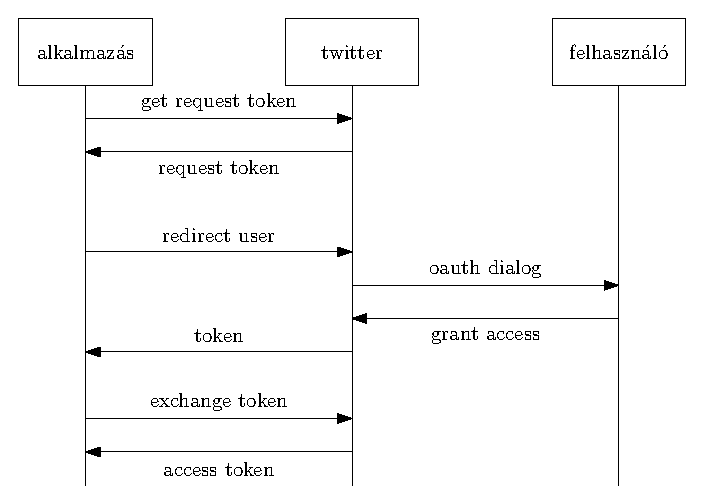
\includegraphics[width=0.95\textwidth]{figures/oauth}
  \caption{A 3-legged OAuth 1.0a autentikációs protokoll}
\end{figure}

Az azonosítás használatához regisztrálni kell a Twitter megfelelő felületén
egy új alkalmazást, majd az ott megkapott adatokkal (tokenekkel)
az autentikáció azonnal használatba vehető.

Az \verb=oauth= modul alternatívája a \verb=passport= modul, ami egy sokkal
általánosabb módszert biztosít felhasználók azonosítására (elérhető teljesen
felkonfigurált Twitter azonosítás is), azonban a \verb=koa= támogatás még
messze nem hibátlan, ezért ennek a használatát végül elvetettem.


\chapter{Tervezés, megvalósítás}

A tervezés során a legfontosabb szempont az architektúra skálázhatósága volt,
hiszen ez elengedhetetlen ahhoz, hogy az alkalmazás valóban képes legyen
elosztott működésre.

A szoftvert ezeknek a követelményeknek megfelelően akartam megtervezni,
el akartam kerülni, hogy \emph{monolitikus} alkalmazást készítsek el,
ehhez a \emph{microservice} architektúra elveit vettem figyelembe,
ami később jó döntésnek bizonyult.

A \emph{monolitikus} és a \emph{microservice} architektúra közül nem lehet
kiválasztani egyértelműen a ``jobb'' megoldást, mindkettőnek vannak előnyei
és hátrányai a másikkal szemben.

\section{Monolitikus architektúra}

Egy \emph{monolitikus} alkalmazás önálló egységet alkot, kompakt, viszonylag
kevés külső függőséggel rendelkezik. Többnyire rétegelt, vagy hexagonális
felépítéssel bír. Ez több előnnyel is jár:

\begin{itemize}
  \item A fejlesztés egyszerű, hiszen a rendelkezésre álló fejlesztőkörnyezetek
    (pl. Visual Studio) ezt a fajta architektúrát támogatják.
  \item Egyszerű az üzemeltetés, hiszen az alkalmazást könnyű deployolni, mivel
    az egyedül is képes a komplett funkcionalitást biztosítani.
  \item Több példányt elindítva a skálázás megoldható, akár automatikusan is,
    ehhez a gyakorlatban csak egy terheléselosztóra van szükség.
\end{itemize}

A hátrányai pont ezek miatt:

\begin{itemize}
  \item A komplex alkalmazások komplex fejlesztőkörnyezetet igényelnek, ami
    megnövekedett erőforrásigénnyel jár.
  \item A komplexitás következtében az alkalmazás nagyon nagy, adott esetben
    az inicializálás ideje nagyon nagyra nőhet, ami a skálázhatóságot rontja.
  \item A skálázási lehetőségek nagyon limitáltak, legtöbb esetben
    erőforráspazarlóak, hiszen az egyetlen lehetőség a több példányos futtatás.
    Ezzel nem csak a szűk keresztmetszetet jelentő komponenst duplikáltuk,
    hanem mindent.
  \item A szoros csatolás miatt megnő a \emph{vendor lock-in} veszélye,
    azaz más technológiára váltás, vagy akár csak egy verziófrissítés
    nagyon komoly kihívást jelent.
  \item Bár egy szakdolgozatban nem okoz problémát, de valódi enterprise
    környezetben egy folyamatban lévő projectbe bekapcsolódás nagyon nehézkes,
    hiszen a fejlesztőnek meg kell értenie az alkalmazást, át kell látnia azt.
\end{itemize}

\section{Microservice architektúra}

A microservice architektúra szinte pontosan az előző ellentéte.
Az egyes szoftverkomponensek önállóan is futtatható alkalmazások,
a futtatáshoz nagyon kevés erőforrásra van csak szükség, a feladatuk
ellátásához azonban szükség van sok másik komponensre.

A komponensek közti kommunikáció valamilyen jól definiált, nyelvfüggetlen
interfészen keresztül zajlik (pl HTTP fölötti JSON kommunikáció, vagy
valamilyen alacsony szintú, TCP/UDP fölött definiált protokoll).

A megoldás előnye, hogy a skálázás sokkal rugalmasabb, elegendő csak a szűk
keresztmetszetet jelentő komponenseket skálázni, így adott esetben
jelentősen kevesebb erőforrás is elengendő a megfelelő szolgáltatási
szint biztosításához.

Az architektúra további előnye, hogy technológiafüggetlen, hiszen az egyes
komponensek teljesen függetlenek egymástól, csak a megfelelő interfészeket
kell biztosítaniuk egymásnak. Egy rétegelt architektúrában ez többnyire nem
megoldható.

Természetesen hátrányok is vannak, az egyik legnyilvánvalóbb, hogy az
üzemeltetés bonyolultabb, amennyiben nem megfelelő eszközöket használunk.
A sok különálló komponens egyenkénti deployolása, illetve konfigurálása
manuálisan nagyon nehézkes, de vannak eszközök, amikkel az egész folyamat
teljesen automatizálható.

\section{Működés felvázolása}

Az alkalmazás két \verb=koa= alkalmazásból, számos apró feldolgozó folyamatból,
és a közöttük üzeneteket továbbító üzenetsorból áll (\emph{queue}),
illetve a külvilág egy \emph{reverse proxy}-n keresztül tud ezekhez hozzáférni.


\begin{itemize}
  \item Egy \verb=koa= alkalmazás bonyolítja le a felhasználóval történő
    kommunikációt (\emph{frontend}).
  \item Egy másik \verb=koa= szerver biztosítja az adatbázishoz a hálózaton
    keresztül történő hozzáférést (\emph{db}).
\end{itemize}

Az egyes alkalmazások, és a köztük lévő kapcsolatok \aref{fig:arch}.
ábrán láthatóak. A komponensek függetlenek az őket futtató környezettől,
így tetszőleges számú (fizikai vagy virtuális) hoszton futtathatóak.

\begin{figure}[h!]
  \centering
  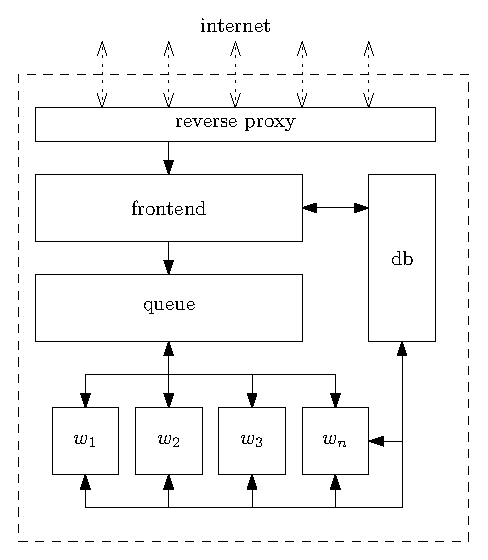
\includegraphics[width=0.6\textwidth]{figures/arch}
  \caption{Az alkalmazás architektúrája}
  \label{fig:arch}
\end{figure}

\section{Frontend alkalmazás}

A felhasználó egy webes felületet lát az alkalmazásból (a design munkákat
ezúton is köszönöm Sári Tamásnak),
a feladata, hogy egy egyszerű SPA-t (Single Page Application) biztosítson,
illetve a különböző interakciókat a megfelelő alrendszereknek továbbítsa.

A frontend szerver egy Nginx \emph{reverse proxy} mögött foglal helyet,
ami a statikus fájlokat (lefordított \verb=stylus= stílusfájlok, illetve
\verb=browserify= bundle-ök, képek) szolgál ki, minden egyéb kérést
a koa szervernek továbbít.

Alapesetben a felhasználó egy statikus HTML oldalra érkezik,
ami csak azért felelős, hogy a CSS stílusfájlok, illetve a kliensoldali JS
állományok betöltődjenek. Ezek után a felhasználó csak AJAX kéréseken keresztül
kommunikál a szerverrel.

A szerver feladata, hogy elindítsa az OAuth autentikációt, a végén keletkező
tokent az adatbázisban eltárolja, valamint beütemezze a megfelelő jobokat,
illetve ha ha ezek befejeződtek, akkor az elkészült statisztikákat
a kliensoldali alkalmazásnak eljuttassa.

\begin{figure}[h!]
  \centering
  \includegraphics[width=0.5\textwidth]{figures/frontend-1}
  \caption{Az alkalmazás kezdő képernyője}
  \label{fig:frontend-1}
\end{figure}

\begin{figure}[h!]
  \centering
  \includegraphics[width=0.5\textwidth]{figures/frontend-2}
  \caption{Az elkészült statisztika grafikonja}
  \label{fig:frontend-1}
\end{figure}

\section{Adatbázis szerver}

Az adatbázis szerver feladata az alkalmazás állapotának számon tartása.
Ezek közé tartozik az egyes \emph{business objektumok} perzisztálása,
illetve ezek menedzselése egy egyszerű REST HTTP JSON interfészen keresztül.

Az üzleti logika szempontjából releváns entitások a következők:

\begin{description}
  \item[user] a felhasználót reprezentáló objektum, a hozzá tartozó
    legfontosabb információkkal (regisztráció időpontja, e-mail cím, stb),
    illetve az elkészült statisztikákat is ebben az objektumban tárolom el.
  \item[token] az egyes Twitter API hívásokhoz szükség van a autentikációs
  tokenekre, ezeket a felhasználótól kapja meg az alkalmazás, az OAuth
  autentikációs során. Fontos számon tartani az állapotát, hányszor lett
  felhasználva, mikor lett utoljára felhasználva.
  \item[tweet] a Twitter API válaszaiból leképzett objektumok, az alkalmazás
  szempontjából az egyetlen releváns adata a tweet időpontja, hiszen ebből
  határozza meg a szoftver az ideális időpontot a tartalom publikálására.
  \item[job] az egyes elvégzendő háttérfeladatok. Az alkalmazás eltárolja a
  a teljes életciklusát, tehát hogy mikor hozták létre, mikor került egy
  feldolgozó egységhez, mikor végzett az vele. Természetesen a job állapota
  is tárolva van, ezzel a többszörös végrehajtást lehet kivédeni.
\end{description}

Egy felhasználó létrehozásakor vele együtt létrejön egy \emph{fetch-followers}
job is, ez indítja be az adott felhasználóhoz tartozó statisztikák
összegyűjtését.

Egy job létrehozásakor nem csak egy adatbázisrekord jön létre, hanem a
hozzá tartozó üzenet bekerül a várakozási sorba (ez az üzenet egyszerűen
a job azonosítóját tartalmazza), amit majd az épp aktív feldolgozóegységek
végrehajtanak.

A felhasználókhoz el van tárolva az aktív, illetve függőben lévő jobok
száma. Mivel ezeket az értékeket inkrementálni kell, amit a LevelDB atomi
műveletként nem támogat, így ezt nekem kellett megvalósítanom.
Ehhez írtam meg a \verb=co-lock= modult, ami kölcsönös kizárást biztosít
erőforrásokhoz, használata pedig a már megszokott \verb=yield= szintaktikával
lehetséges:

\begin{js}
  var lock = require('co-lock');

  var release = yield lock(resource);
  // kritikus szakasz
  yield release;
\end{js}

A háttérben a modul a \verb=resource= erőforráshoz egy zárat hoz létre,
vagy ha az már zárolva van, akkor annak a \emph{várakozási sorába} lép be,
a \verb=yield release= ezt a zárat engedi el, azaz a várakozási sorban
következő hívás hajtódik végre.

Zárak használatakor ügyelni kell a \emph{deadlock} elkerülésére.
Szerencsére az alkalmazásban máshol nem volt szükség zárakra, ezért
a deadlock nem fordulhat elő (hiszen ahhoz több erőforrásra van szükség,
az adatbázis azonban műveletenként csak egyet használ).

\section{Aszinkron üzenetsor}

A service felelőssége, hogy az egyes elvégzendő feladatokat ütemezze,
és azok a megfelelő feldolgozóegységekhez eljuttassa.

A működés során fontos, hogy az üzenetek ne vesszenek el (pl. ha a
szolgáltatás újraindul), ehhez szükség van a megfelelő kommunikációs és
tranzakciós protokollokra. Mivel ezek megvalósítása a gyakorlatban sok
körültekintést igényel, így elvetettem a saját megoldás implementálásának
lehetőségét.

A RabbitMQ szoftvert választottam a feladatra, ami az AMQP specifikációt
implementáló Erlang-alapú szoftver. Az egyes szoftverkomponensek egy RabbitMQ
szerveren keresztül kommunikálnak, így ha egy szolgáltatás rövid időre leáll,
akkor a függőben lévő üzenetek a szerveren tárolódnak (természetesen itt is
perzisztensen, így a RabbitMQ szerver leállása vagy meghibásodása esetén sem
kell tartani az adatvesztéstől).

A szerver feladata elsősorban az üzenetek továbbítása, azonban az üzenetsor
működésének jellegét kihasználva egy \emph{resource pool}-t is megvalósítottam
vele. Az egyes feladatok elvégzéséhez szükség van \emph{tokenekre}, melyek
segítségével autentikált Twitter API hívások végezhetők, mivel azonban ezek
használata erősen korlátozott (adott időintervallumban csak bizonyos számú
API hívás végezhető el), így meg kell akadályozni, hogy az egyes tokenek
``kimerüljenek'', azaz kölcsönös kizárást kell biztosítani hozzájuk,
azokat csak meghatározott időközönként lehet újra felhasználni.
A vázlatos működés \aref{fig:queue}. ábrán látható.

\begin{figure}[h!]
  \centering
  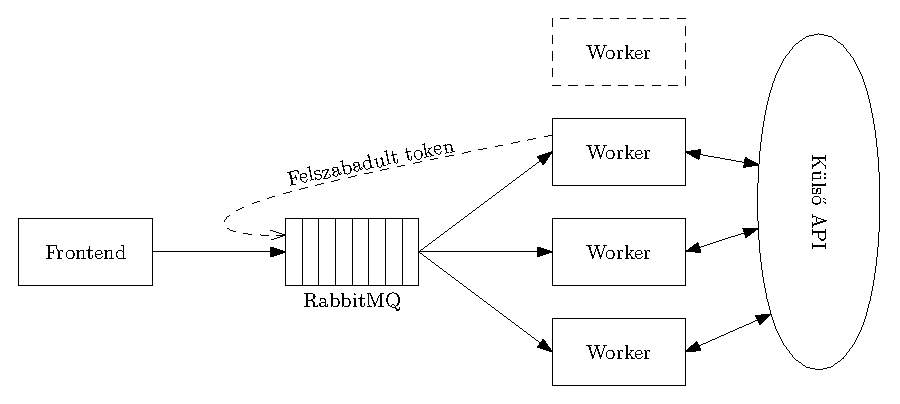
\includegraphics[width=0.95\textwidth]{figures/queue}
  \caption{Az üzenetsor szerepe az alkalmazásban}
  \label{fig:queue}
\end{figure}

\subsection{AMQP}

Az AMQP (Advanced Message Queuing Protocol) egy rugalmas protokoll üzenetek
változatos minták szerinti továbbítására. A \emph{termelők} a szerverhez
kapcsolódva egy \emph{exchange}-ben publikálják az üzenetüket,
a szerver pedig az üzenet \emph{routing key}-e
(és az aktuális \emph{exchange-queue bindingok}) alapján továbbítja a
megfelelő \emph{queue(k)}-ba. A \emph{fogyasztók} az egyes queue-kra
iratkoznak fel, a szerver pedig továbbítja az üzenetet egy (vagy több)
fogyasztónak.

Az elkészült alkalmazás nem használ bonyolult mintákat, minden üzenet
az alapértelmezett exchangen keresztül publikálódik, a routing key pedig
megegyezik a queue nevével, ami pedig az adott feladat nevével egyezik meg,
így az egyszerűség kedvéért a továbbiakban az üzenet publikálás alatt
azt lehet érteni, hogy megérkezik a routing key-nek megfelelő queue-ba az
üzenet.

\subsection{Resource pool}

Az egyes tokenek felhasználása korlátozott, így a befejezett feladat után
nem szabad azt rögtön visszarakni a pool-ba, hanem bizonyos ideig
``várakoztatni'' kell.

Ezt egy közbenső queue beiktatásával oldom meg. Az AMQP protokol támogatja,
hogy az egyes üzenetekhez TTL-t (Time to Live) rendeljünk.
Ha az üzenetet nem sikerült ezen idő alatt eljuttatni egy fogyasztóhoz,
akkor automatikusan \emph{dead} állapotú lesz. Ha a queue-nak beállítunk
ún. \emph{dead-letter-exchange}-t, akkor ezek az üzenetek kiürülnek az
üzenetsorból, és újra publikálódnak a megadott exchange-n, a megadott
routing key-el (\emph{dead-letter-routing-key}).

Ezt kihasználva, használat után az egyes tokenek egy olyan queue-ba kerülnek,
aminek nincsenek fogyasztói, ezért a megfelelő idő eltelte után újra
visszakerülnek a pool-ba. A működés \aref{fig:pool}. ábrán látható.

\begin{figure}[h!]
  \centering
  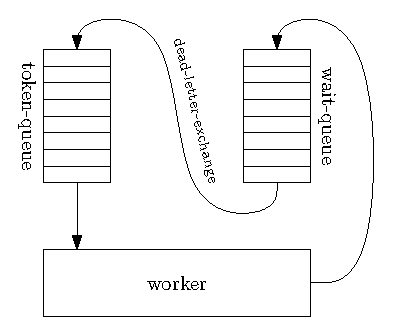
\includegraphics[width=0.6\textwidth]{figures/pool}
  \caption{Resource pool megoldás}
  \label{fig:pool}
\end{figure}

Mivel a TTL a queue-ra nézve állandó (létezik az üzenetre értelmezett TTL is,
de az nem használható az általam elérni kívánt funkcionalitáshoz), így
minden TTL-hez külön queue-t kell deklarálni.
Erre hoztam létre az \verb=amqp-schedule= modult. A könyvtár egy egyszerű
interfésszel elrejti előlünk ezt az ideiglenes üzenetsort:

\begin{js}
  var scheduler = require('amqp-schedule');
  var publish = scheduler(conn); // conn: amqp kliens objektum

  publish(exchange, key, message, delay, opts, cb);
  // vagy
  publish(exchange, key, message, date, opts, cb);
\end{js}

A késleltetés a \verb=delay= paraméterrel szabályozható, vagy konkrét időpont
(\verb=date=) is megadható. A háttérben egy speciálisan elnevezett
queue jön létre, ami a megfelelő \emph{dead-letter-exchange},
\emph{dead-letter-routing-key} és \emph{message-ttl} paraméterekkel rendelkezik,
azaz a megadott idő után az üzenet automatikusan a cél queue-ba kerül.
Mivel az eltérő időzítések új üzenetsorokat hoznak létre, így
a létrejött ideiglenes queue-k rendelkeznek \emph{expires} paraméterrel,
ami azt szabja meg, hogy mennyi \emph{idle} idő (üresjáratban töltött)
után szűnjenek meg maguktól. Így a szerver védve van attól, hogy a már nem
használt, üres üzenetsorok erőforrásokat foglaljanak.

\section{Háttérfolyamatok}

\begin{figure}[h!]
  \centering
  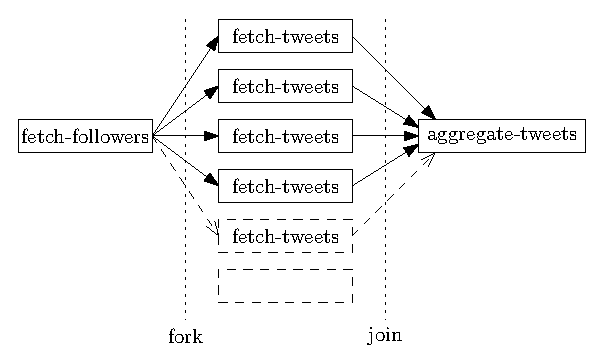
\includegraphics[width=0.75\textwidth]{figures/workflow}
  \caption{Az alkalmazásban lévő háttérfolyamatok összefüggései}
  \label{fig:workflow}
\end{figure}

Az egyes háttérfolyamatok egyszerű Node.JS alkalmazások, amik csatlakoznak
a RabbitMQ szerverhez, és egy adott típusú feladatot végeznek el.

Tetszőleges számú példány elindítható, a kommunikáció hálózaton keresztül
zajlik, így amíg hozzáférnek az üzenetsorhoz, illetve az adatbázishoz,
addig lényegtelen, hogy milyen környezetben futnak.

Alapvetően három fajta feladatot definiáltam, ezek összefüggései
\aref{fig:workflow}. ábrán láthatóak. A feladatok végrehajtásának sorrendje
nem kötött, azonban az egyes folyamatoknam szükségük van egy ponton
szinkronizációra, ennek megoldása nem triviális feladat.

\subsection{Job elosztás}

Az egyes elvégzendő feladatokat a RabbitMQ osztja szét a kliensek között,
akik egymástól teljesen függetlenül képesek működni párhuzamosan,
akár több futtató gépen is.

Az AMQP protokoll támogatja az üzenetek kézbesítésének visszaigazolásos módját,
azaz egy üzenet a célba juttatás esetén csak \emph{unacked} állapoba kerül,
azt a kliensek kell visszaigazolnia. Ezt a kliens az adott feladt elvégzése
után teszi meg, ha a feladatot nem sikerül elvégezni (mert a kliens ezt
explicit kijelenti, vagy a kapcsolat a klienssel megszakad), akkor
az üzenet automatikusan újraütemeződik.

Az AMQP Node.JS binding nem támogatja az üzenetek egyesével történő
elfogyasztását, így az általam használt megoldás egy feliratkozásból,
és egy leiratkozásból áll:

\begin{js}
function* peek(queue) {
  var done;
  var tag;
  queue.subscribe({
    ack: true,
    prefetchCount: 1,
  }, function(message, headers, deliveryInfo, job) {
    queue.unsubscribe(tag).addCallback(function() {
      done(null, {
        message: message,
        headers: headers,
        deliveryInfo: deliveryInfo,
        job: job,
      });
    });
  }).addCallback(function (ok) {
    tag = ok.consumerTag;
  });
  return yield function(cb) {
    done = cb;
  };
}
\end{js}

A feliratkozáskor a kliens egy ún. \emph{consumer tag}-et kap,
ami a feliratkozást azonosítja. Az üzenetek \emph{ack} módban érkeznek,
azaz amíg \verb=prefetchCount= számú üzenet nincs visszaigazolva,
addig a nem kap több üzenetet a kliens.

Ha az első üzenet megérkezett, akkor a kliens az eltárolt consumer tag
alapján elvégzi a leiratkozást, és a hívónak visszaadja a kapott üzenetet,
illetve a hozzá tartozó metaadatokat. Ha a hívó elvégezte a feladatát,
a \verb=job.acknowledge()= metódussal visszaigazolja az üzenetet,
vagy a \verb=job.reject(requeue)=-tel eldobja (és a paraméter értékétől
függően újra beálltja az üzenetsorba).

\subsection{fetch-followers}

A feldolgozás első lépése, hogy a felhasználó követőit lekérdezzük a Twitter
API-ból.

Az API válasz hatására minden egyes követőhöz hozzá kell rendelni
(és beütemezni) egy \emph{fetch-tweets} feladatot,
ami majd az egyes felhasználók tweetjeit fogja megszerezni.

Egy API kérés maximum 1500 követőt képes visszaadni, így ennél nagyobb
mennyiségnél újabb \emph{fetch-followers} feladatot kell beütemezni,
így a \emph{fetch-followers} rekurzívan szerzi meg a felhasználó követőit.

\subsection{fetch-tweets}

A \emph{fetch-tweets} egy adott felhasználó legutolsó tweetjeit kérdezi le,
egy adott időponttól kezdve. A tervezés során úgy határoztam, hogy az egyes
felhasználóknak csak az utolsó két hétben publikált tweetjeit kérdezem le,
vagy amennyit a rendszer megenged (3200 tweet, szerencsére ez minden
esetben elegendőnek bizonyult).
Kezdetben a legutolsó 200 tweetet kérdezi le a rendszer,
majd ha ezek közül egyik tweet sem régebbi 2 hétnél,
akkor a készít egy új \emph{fetch-tweets} jobot, ami a legrégebbi
(de még mindig két hétnél frissebb) tweet előtti üzeneteket tölti le.
Így előbb-utóbb rekurzív módon minden szükséges tweet letöltésre kerül.

\subsection{aggregate-tweets}

Ha az adatok begyűjtése megtörtént, akkor a rendszer elvégzi az összegyűjtött
tweetek aggregálását. A folyamat egyrészt detektálja, hogy valóban el kell-e
végezni az aggregálást (azaz a felhasználónál nem maradt már \emph{pending}
állapotú feladat): ha még további adatok letöltése szükséges,
akkor befejezi a futást.
Amint az utolsó job is lefutott, megtörténik a tényleges aggregálás.
Ehhez le kell kérdezni az adatbázisból az összegyűjtött tweeteket, majd
azokat csoportosítani a létrehozásuk ideje alapján, végül az ezekbe a
csoportokba eső üzeneteket kell megszámolni. Az eredményt el kell tárolni,
hogy azt a frontend alkalmazás a felhasználónak később meg tudja mutatni.

\section{Naplózás}

A naplózást minden rendszer saját hatáskörében végzi el, azonban azokat
egy közös helyre (InfluxDB) is beteszi. Így az adatok központilag elemezhetők,
de lebonthatóak alkalmazásokra, hosztokra, folyamatokra.

\subsection{HTTP kérés naplózás}

A frontend szerver egyszerűen a beérkező HTTP kéréseket naplózza, ezek
válaszidejét méri. Ez a gyakorlatban az OAuth-tal összefüggő kéréseket
jelenti.

\subsection{Adatbázis naplózás}

Az adatbázis külön naplóz minden adathozzáférést, annak típusa szerint
csoportosítva (írás, olvasás), illetve az erőforrás típusa (tweet, user, stb.)
alapján. Ezen felül a HTTP interfészének válaszidejét is méri, így
külön-külön mérhető az adatbázis, illetve a szerver válaszideje
(a szerver válaszideje ekkor az adatbázis és a
HTTP szerver \emph{overhead}jének összege).

\subsection{Háttérfolyamatok}

Az egyes végrehajtó folyamatok is monitorozzák az általuk végrehajtott
feladatokat

\begin{itemize}
  \item Mennyi idő alatt hajtotta végre az adott feladatot
  \item Mekkora volt a Twitter API válaszideje
  \item Mennyi időt töltött a várakozási sorban, amíg sorra került
  \item Hiba esetén naplózni kell a hiba eredetét (adatbázishiba,
    vagy a Twitter hibája)
\end{itemize}

A feldolgozás során a Twitter számos hibát generál. Ezek túlnyomó többsége
a privát Twitter felhasználók miatt van: az ő tweetjeit csak bizonyos
emberek láthatják (akiknek előzetesen jóváhagyta), így ezeket az üzeneteket
az API-ból sem tudjuk elérni. Ilyenkor jobb megoldás híján az adott
\emph{fetch-tweets} jobot befejezettnek tekintjük.

Fel kell készülni az olyan hibákra is, hogy az API (vagy éppen az adatbázis)
elérhetetlen: ilyenkor a jobot nem szabad lezárni, újra be kell ütemezni.
Ez praktikusan egy \verb=job.reject(true)= hívással történik meg, azaz
a feladat visszakerül a feldolgozási sor elejére.


\chapter{Eredmények, továbbfejlesztési lehetőségek}

\section{Mérési adatok}

Az elkészült szoftverrel analizáltam 11000 Twitter felhasználó tweetjeit,
közben figyelemmel kísértem a szoftver teljesítményét.

Az adatbázis a futás során másodpercenként 20 kérést szolgált ki,
ez túlnyomórészt írási művelet (\ref{fig:req-per-sec}. ábra).

Az adatbázis válaszideje meglepően magas volt, hét párhuzamosan futó worker
folyamat mellett 200ms körüli értékeket mutatott, ez feltehetően a sor
járulékos műveletre vezethető vissza (számláló inkrementálás).
A válaszidőket \aref{fig:mean-db-time}. ábra mutatja.

\begin{figure}[h!]
  \centering
  \includegraphics[width=0.9\textwidth]{figures/req-per-sec}
  \caption{Adatbázis kérések száma 10 másodperces időablakokban}
  \label{fig:req-per-sec}
\end{figure}

\begin{figure}[h!]
  \centering
  \includegraphics[width=0.9\textwidth]{figures/mean-db-time}
  \caption{Átlagos adatbázis válaszidő 7 worker folyamat mellett (ms)}
  \label{fig:mean-db-time}
\end{figure}

\Aref{fig:queue-progress}. ábrán az üzenetsor állapota látható a
\emph{fetch-followers} futása során. Ekkor kerülnek beütemezésre az egyes
felhasználók tweetjeit lekérdező jobok \emph{fetch-tweets}.

\begin{figure}[h!]
  \centering
  \includegraphics[width=0.6\textwidth]{figures/queue-progress}
  \caption{A fetch-tweets feladatok felhalmozódása}
  \label{fig:queue-progress}
\end{figure}

Az egyes worker folyamatok teljesítményét szintén nyomon tudtam
követni.
\Aref{fig:mean-twitter}. ábrán a Twitter API átlagos válaszideje,
\aref{fig:mean-worker}. ábrán pedig az egyes jobok átfutási ideje látható.
Leolvasható, hogy a külső szolgáltatás viszonylag gyors,
a szűk keresztmetszetet az adatbázis jelenti.

\begin{figure}[h!]
  \centering
  \includegraphics[width=0.9\textwidth]{figures/mean-twitter}
  \caption{A Twitter API átlagos válaszideje (ms)}
  \label{fig:mean-twitter}
\end{figure}

\begin{figure}[h!]
  \centering
  \includegraphics[width=0.9\textwidth]{figures/mean-worker}
  \caption{A jobok átlagos feldolgozási ideje (ms)}
  \label{fig:mean-worker}
\end{figure}

Az adatbázis sebessége az aggregációs fázisban nagyságrendekkel jobb,
átlagosan 15ms (\ref{fig:mean-read}. ábra). A folyamat során több mint
egy millió tweet került feldolgozásra.

\begin{figure}[h!]
  \centering
  \includegraphics[width=0.9\textwidth]{figures/mean-read}
  \caption{Átlagos válaszidő olvasás esetén (ms)}
  \label{fig:mean-read}
\end{figure}

\input{3_improve}
\section{Összefoglalás}

A tervezés során felvázolt microservice architektúra sikeresnek bizonyult,
az egyes komponensek képesek voltak egymástól és a futtató környezettől
függetlenül üzemelni, a feldolgozó egységek számának változtatásával
a skálázás nagyon finoman állítható be.

A rendszer képes robusztusan, hibatűrően működni, a rendszerben előforduló
hibákra fel van készülve, egyes szoftverkomponensek kiesése esetén
sem omlik össze, a hiba elhárultával zavartalanul képes tovább működni.

A szűk keresztmetszet a szoftverben egyértelműen az adatbázis, ezen
a jobban megválasztott adatszerkezetek, illetve a hatékonyabb adatfeldolgozás
segíthetne.



\listoffigures\addcontentsline{toc}{chapter}{Ábrák jegyzéke}
% \listoftables\addcontentsline{toc}{chapter}{Táblázatok jegyzéke}

\bibliography{bib/mybib}
\addcontentsline{toc}{chapter}{Irodalomjegyzék}
\bibliographystyle{plain}

A hivatkozott internetes források utolsó hozzáférési ideje: \today

\label{page:last}
\end{document}
